\documentclass[12pt]{article}

\textheight=24cm %высота текста
\textwidth=16cm %длина текста
\oddsidemargin=0pt %отступ от левого края
\topmargin=-1.5cm %отступ от верхнего края
\flushbottom %выравнивание высоты страниц

\usepackage[utf8]{inputenc}
\usepackage[T2A]{fontenc}
\usepackage{tikz}
\usepackage{amsmath}
\usepackage{url}
\usepackage[russian]{babel}


\def\d#1#2{\frac{\partial#1}{\partial#2}}
\def\dd#1#2{\frac{\partial^2 #1}{\partial#2^2}}

\title{Второе задание курса 'Суперкомпьютерное моделирование и технологии программирования'}
\date{2018\\ Ноябрь}
\author{Чаплыгин Андрей Викторович\\  ВМК МГУ, группа 603.}

\begin{document}
\maketitle
\section{Описание задачи}
{\bf Вариант 10.} 

В прямоугольнике $\Omega = [0, 2] \times [0, 1]$ с границами:
$$ \gamma_R = \{(2, y), 0 \leq y \leq 1 \} $$
$$ \gamma_L = \{(0, y), 0 \leq y \leq 1 \} $$
$$ \gamma_T = \{(x, 1), 0 \leq x \leq 2 \} $$
$$ \gamma_B = \{(x, 0), 0 \leq x \leq 2 \} $$
рассматривается уравнение Пуассона:
$$ -\Delta u = -(\dd{u}{x} + \dd{u}{y}) = F(x, y) $$
с граничными условиями:
$$ \gamma_R: u(2, y) = \phi(2, y) = 1 + \cos(2 \pi y) $$
$$ \gamma_L: \d{u}{x}_{x=0} = \psi(0, y) = 0 $$
$$ \gamma_T: u(x, 1) = \phi(x, 1) = 1 + \cos(\pi x) $$
$$ \gamma_B: \d{u}{y}_{y=0} = \psi(x, 0) = 0 $$
И правой частью $F(x, y) = \cos(\pi x y) ((\pi y)^2 + (\pi x)^2)$.

Аналитическое решение этой задачи известно:
$$ u(x, y) = 1 + \cos(\pi x y) $$

\section{Численное решение}
Определим равномерную прямоугольную сетку с шагами по пространству $h_x, h_y$. 
Количество узлов сетки $M, N$. Тогда разностная схема решения выглядит следующим образом:

$$ -\frac{1}{h_x^2} (u_{i+1, j} - 2u_{i, j} + u_{i-1, j}) 
   -\frac{1}{h_y^2} (u_{i, j+1} - 2u_{i, j} + u_{i, j-1}) = F_{i, j}, 
   i = \overline{1, M-1}, j = \overline{1, N-1} $$

$$ -\frac{1}{h_x^2} (u_{i+1, 0} - 2u_{i, 0} + u_{i-1, 0}) 
   -\frac{2}{h_y^2} (u_{i, 1} - u_{i, 0}) = F_{i, 0} - \frac{2}{h_y} \psi_{i, 0}, 
   i = \overline{1, M-1}, j = 0 $$

$$ -\frac{2}{h_x^2} (u_{1, j} - u_{0, j}) 
   -\frac{1}{h_y^2} (u_{0, j+1} - 2u_{0, j} + u_{0, j-1}) = F_{0, j} - \frac{2}{h_x} \psi_{0, j}, 
   i = 0, j = \overline{1, N-1} $$   
  
$$ -\frac{2}{h_x^2} (u_{1, 0} - u_{0, 0}) 
   -\frac{1}{h_y^2} (u_{0, 1} - u_{0, 0}) = F_{0, 0} - (\frac{2}{h_x} + \frac{2}{h_y}) \psi_{0, 0} $$
   
$$ u_{M, j} = \phi_{M, j}, j = \overline{0, N} $$

$$ u_{i, N} = \phi_{i, N}, i = \overline{0, M} $$

Полученную систему линейных уравнений предлагается решать методом наименьших невязок.

\newpage 

\section{Программная реализация}
\subsection{Описание последовательной версии}
Представим нашу разностную схему в матричном виде:
$$ L u = G $$
Заметим, что размерность $L \in R^{MN \times MN}$, т.к. на границах $\gamma_R, \gamma_T$ задаются условия Дирихле
и узлы на этой границе можно исключить из системы.

Т.к. в методе наименьших невязок только требуется вычислять $Lv$ для вообще говоря произвольного
$v$ - то в программе реализован безматричный вариант метода (matrix-free). 
Вместо построения матрицы оператора $L$ задается функция, вычисляющая $Lv$ по заданному вектору $v$ (matvec).

В качестве критерия остановки итерационного процесса использовался критерий: 
$$||r_k|| = ||Lu_k - G|| < \epsilon $$

Последовательная версия лежит в git репозитории: 
\url{https://github.com/Andrcraft9/laplace2D-solver}, ветка master

\subsection{Описание параллельной версии (MPI и OpenMP)}
При параллельной реализации использовался метод декомпозиции области.
Область делилась в двух направлениях: по x и по y.
Для каждой подобласти добавлялась внерасчетная граница (halo points), 
с помощью которой происходила синхронизация между процессорами.
В качестве функций перессылок использовались MPI блокирующие вызовы 
MPI\_Sendrecv, MPI\_Send, MPI\_Recv.

С помощью директив OpenMP были распараллелены главные циклы программы.

\bigskip

MPI версия программы лежит в git репозитории: 
\url{https://github.com/Andrcraft9/laplace2D-solver}, ветка pure\_mpi

Гибридная MPI/OpenMP версия программы лежит git репозитории: 
\url{https://github.com/Andrcraft9/laplace2D-solver}, ветка parallel\_mpi

\newpage

\section{Тестирование последовательной программы и параллельной программы}

\subsection{Тестирование на персональном компьютере}

Тестирование проводилось на персональном компьютере с процессором
Intel(R) Core(TM) i7-7700HQ CPU @ 2.80GHz, $\epsilon = 10^{-6}$.

Приведем сначала результаты последовательной программы.
\begin{center}
\begin{tabular}{lllllll}1
Mesh & Time (sec) & Iterations & Error (L2) & Error (C) \\
\hline
20 x 20 & 0.005695 & 570 & 0.040182 & 0.005018 \\
40 x 40 & 0.147708 & 4949 & 0.019857 & 0.001262 \\
80 x 80 & 1.393880 & 33370 & 0.009860 & 0.000316 \\
160 x 160 & 23.535339 & 153615 & 0.004905 & 0.000079 \\
\hline
\end{tabular}
\end{center}
Из таблицы четко видно, что при увеличении сетки в два раза ошибка в норме L2 падает
в 2 раза, а в норме C в 4 раза. Приведем рисунки как ведет себя
численное решение на итерациях для двух сеток.

\begin{figure}[htb!]
\begin{minipage}[h]{0.49\linewidth}
\center{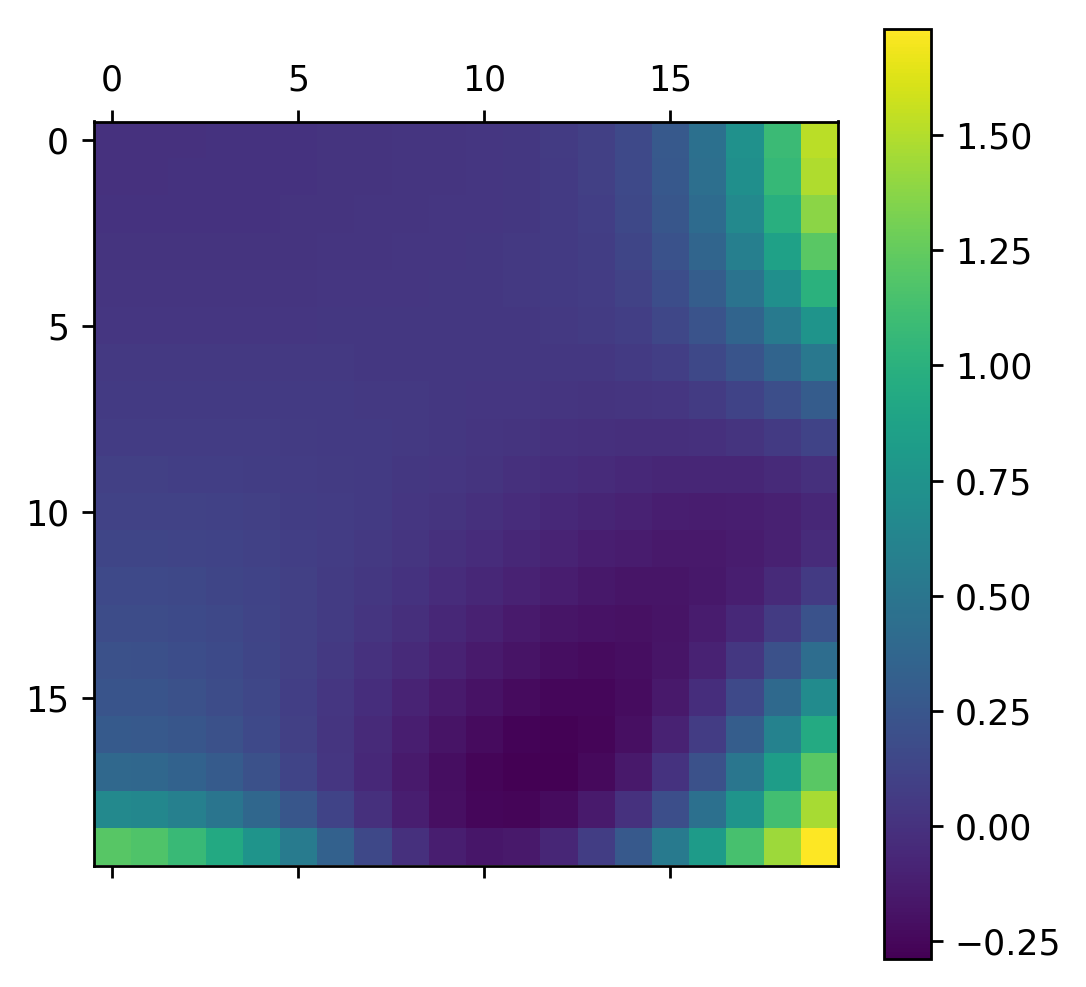
\includegraphics[scale = 0.5]{./figs/20/results_10.png}}
\end{minipage}
\hfill
\begin{minipage}[h]{0.49\linewidth}
\center{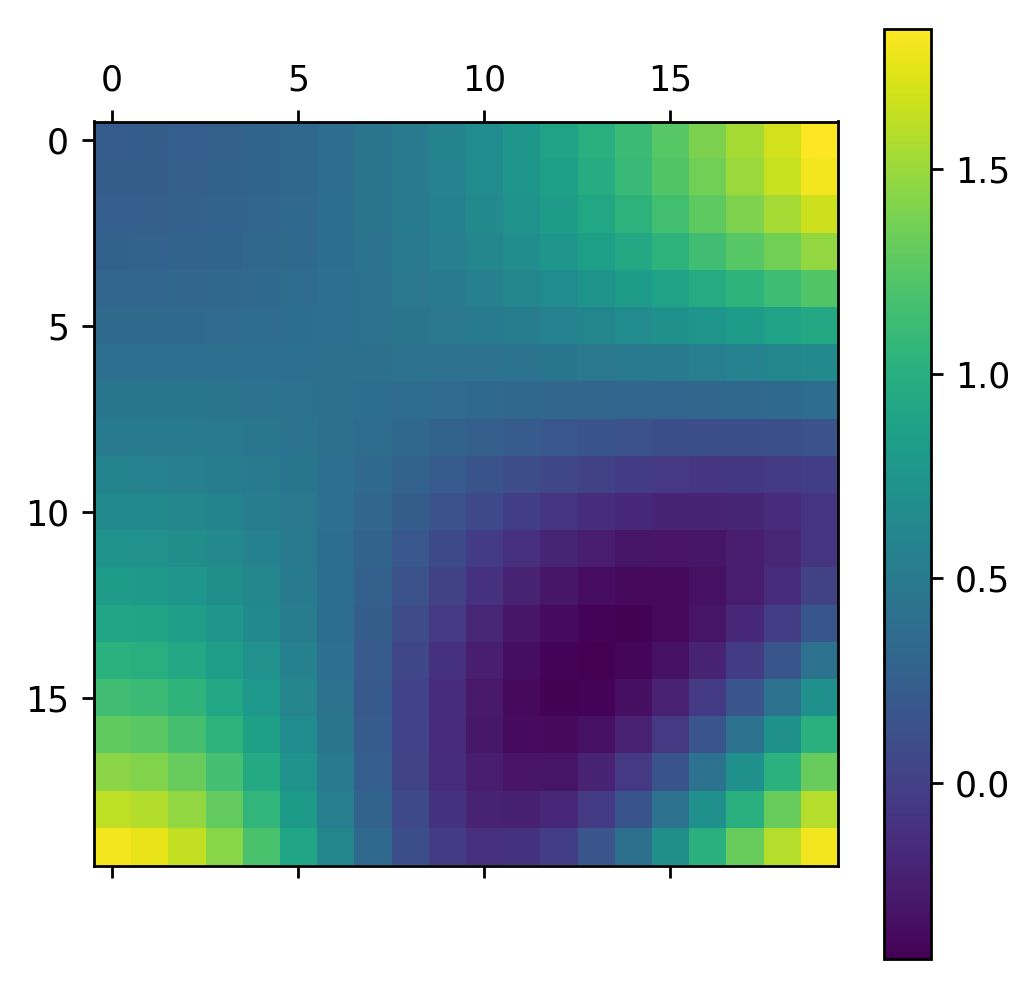
\includegraphics[scale = 0.5]{./figs/20/results_100.png}}
\end{minipage}
\caption{Решение для сетки 20 на 20: слева на 10 итерации; справа на 100 итерации}
\end{figure}

\begin{figure}[htb!]
\begin{minipage}[h]{0.49\linewidth}
\center{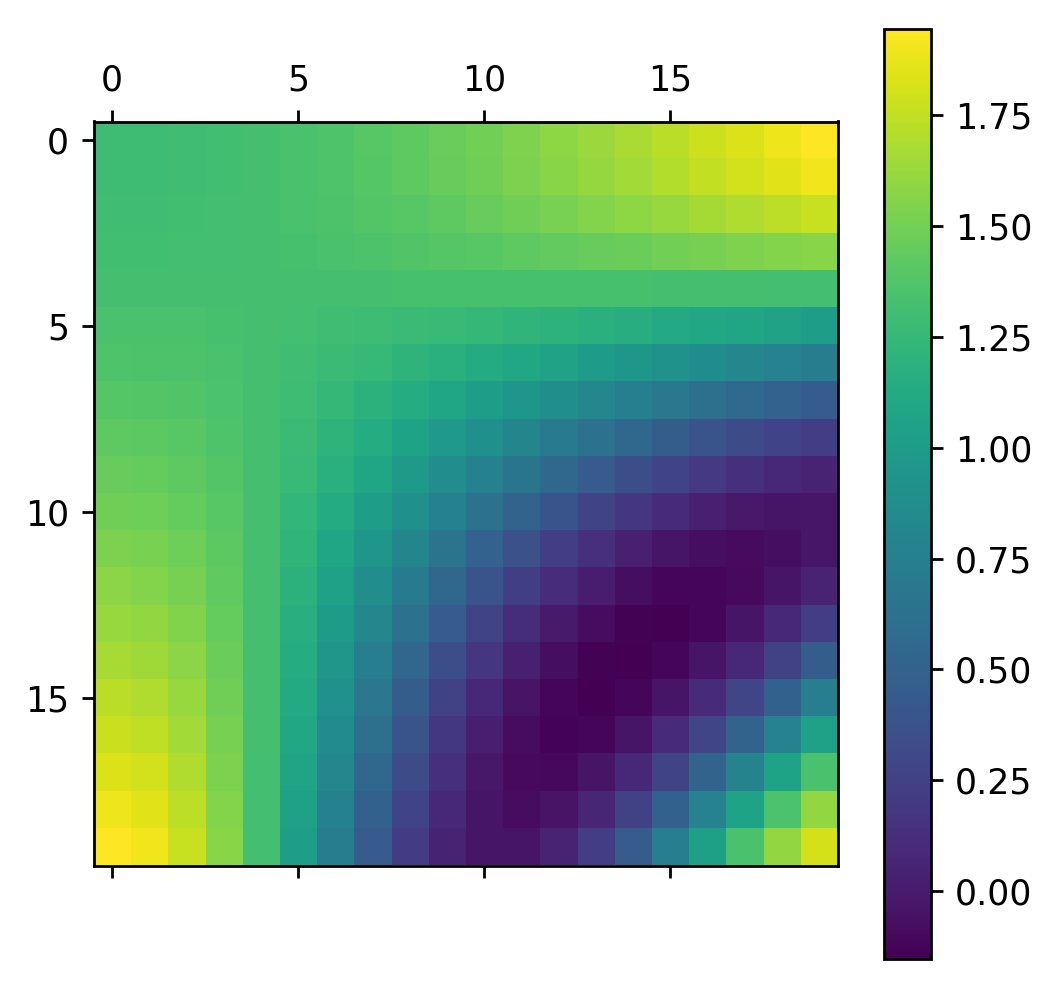
\includegraphics[scale = 0.5]{./figs/20/results_300.png}}
\end{minipage}
\hfill
\begin{minipage}[h]{0.49\linewidth}
\center{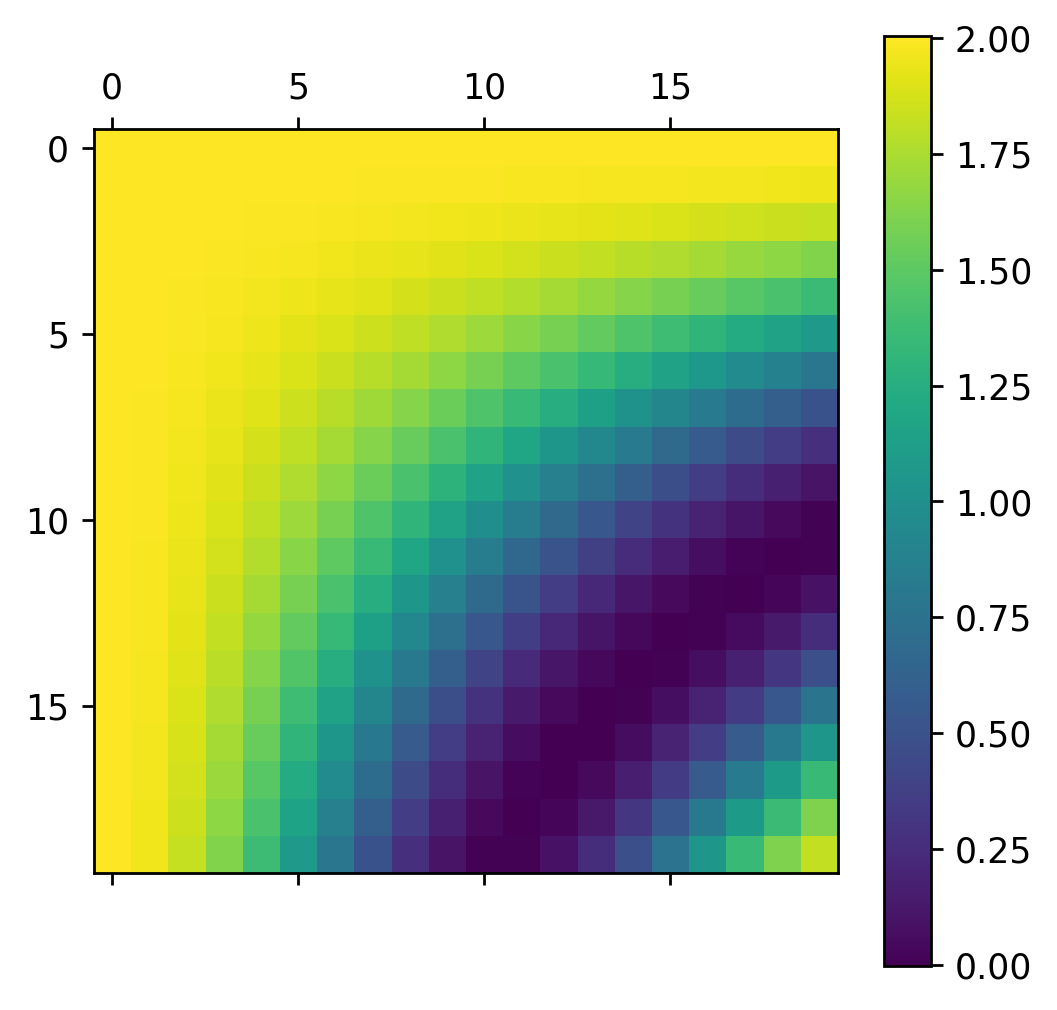
\includegraphics[scale = 0.5]{./figs/20/results_final.png}}
\end{minipage}
\caption{Решение для сетки 20 на 20: слева на 300 итерации; справа финальное (570 итерация)}
\end{figure}

\begin{figure}[htb!]
\begin{minipage}[h]{0.49\linewidth}
\center{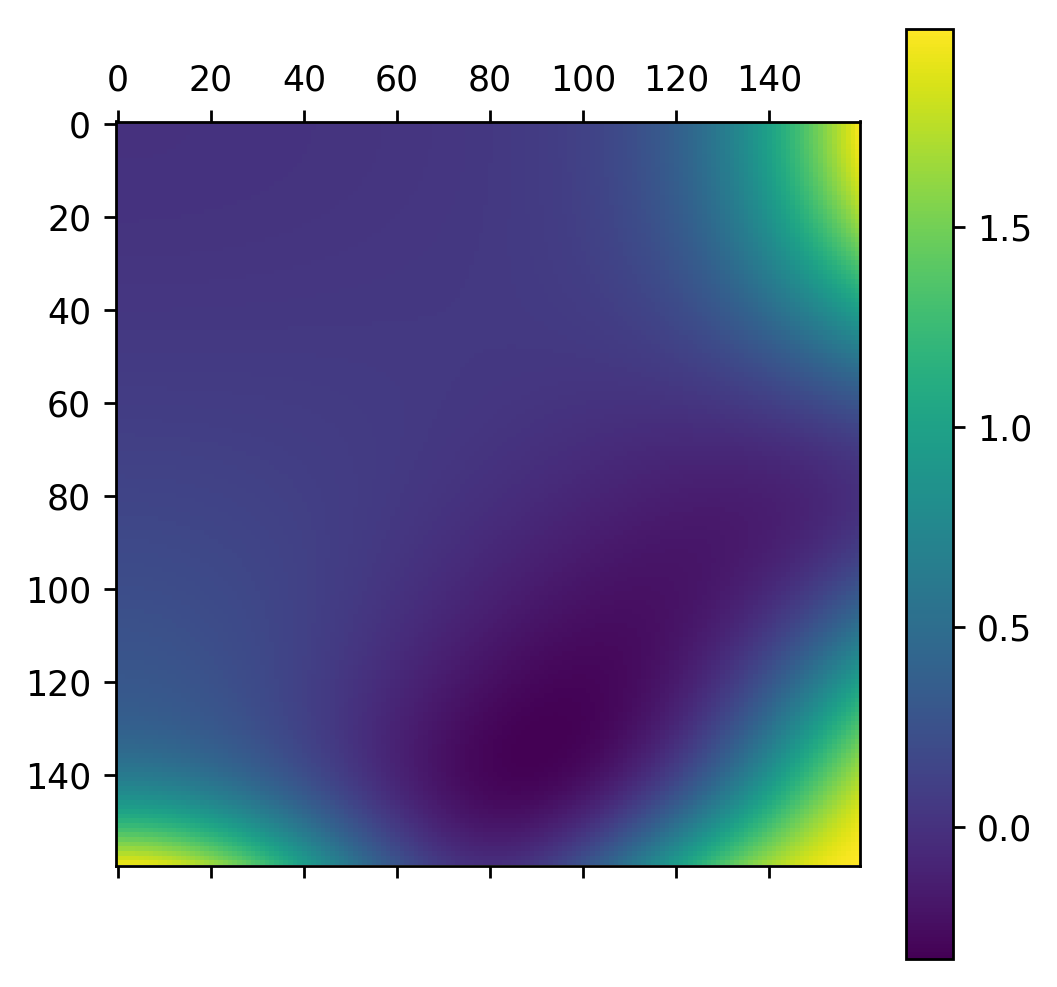
\includegraphics[scale = 0.5]{./figs/160/results_1000.png}}
\end{minipage}
\hfill
\begin{minipage}[h]{0.49\linewidth}
\center{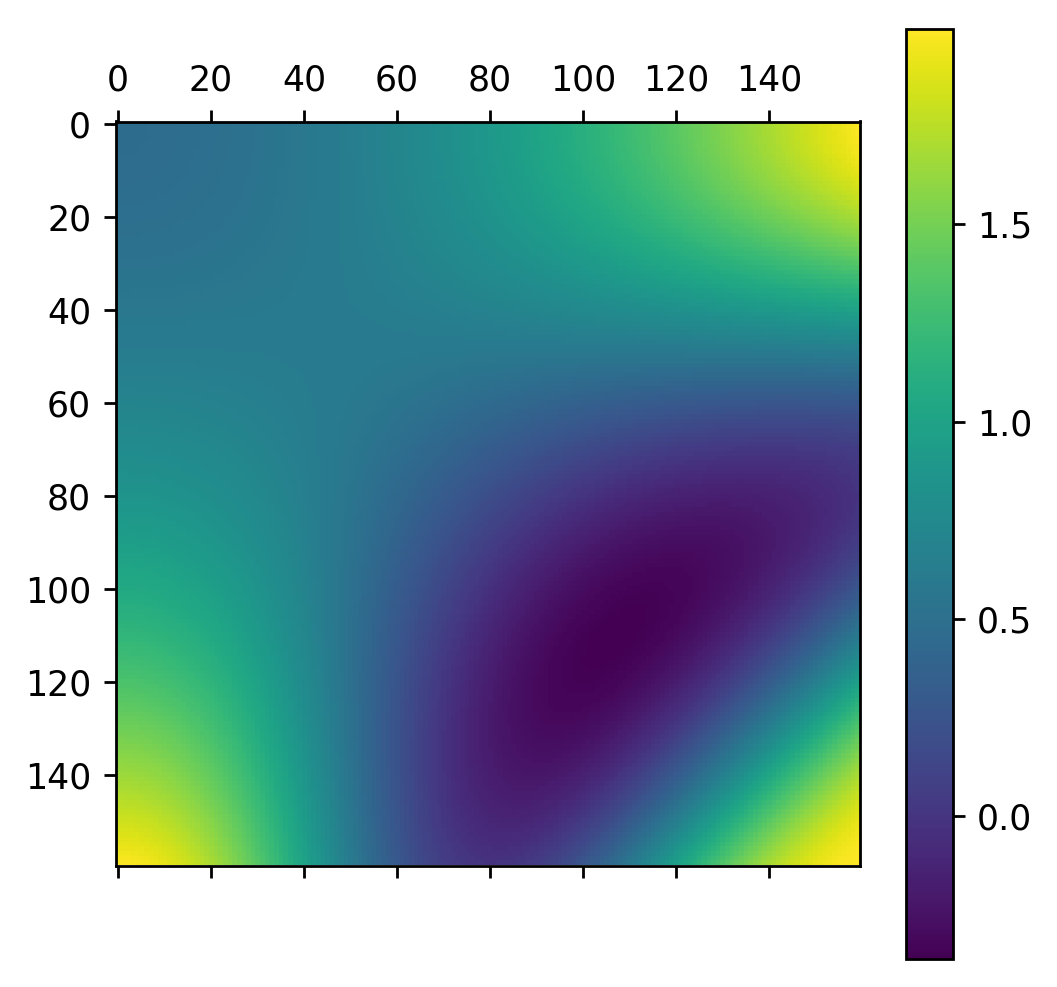
\includegraphics[scale = 0.5]{./figs/160/results_10000.png}}
\end{minipage}
\caption{Решение для сетки 160 на 160: слева на 1000 итерации; справа на 10000 итерации}
\end{figure}

\begin{figure}[htb!]
\begin{minipage}[h]{0.49\linewidth}
\center{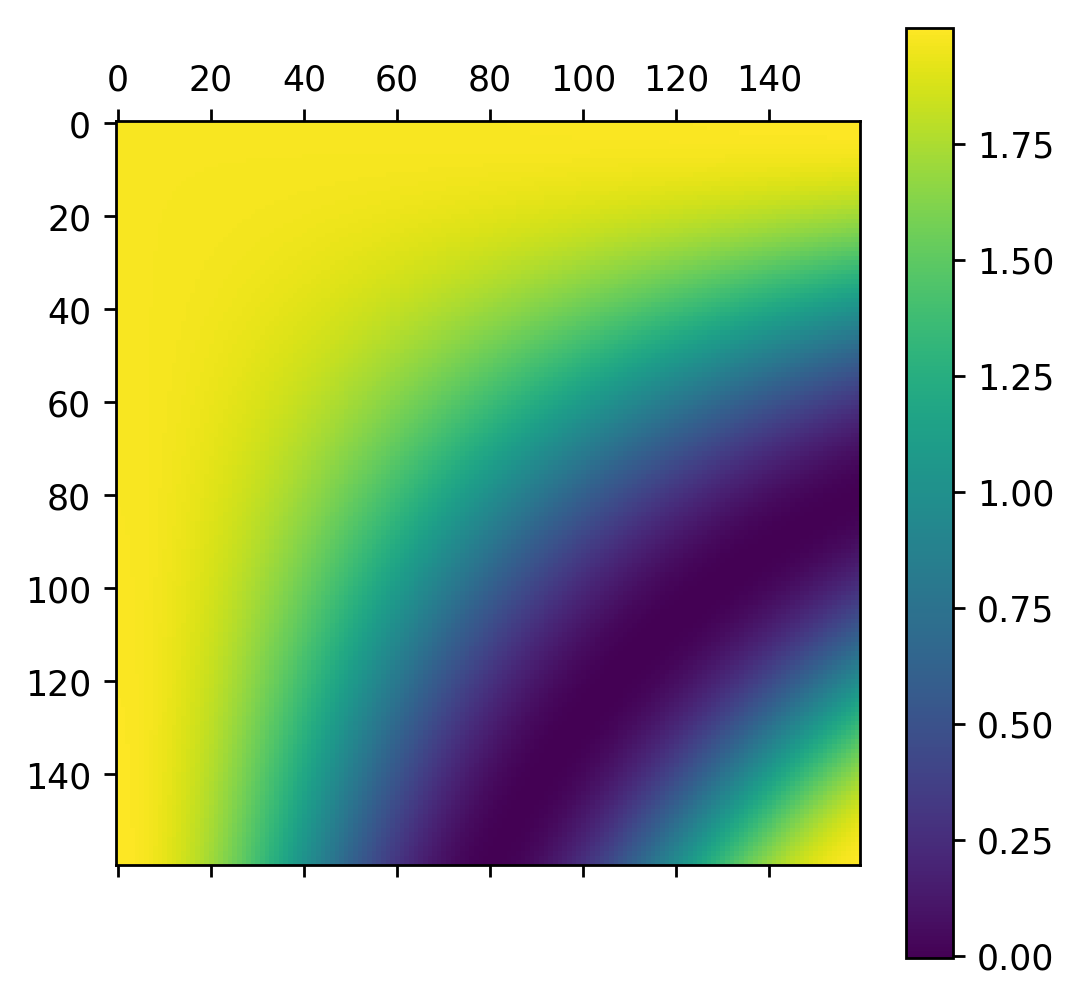
\includegraphics[scale = 0.5]{./figs/160/results_50000.png}}
\end{minipage}
\hfill
\begin{minipage}[h]{0.49\linewidth}
\center{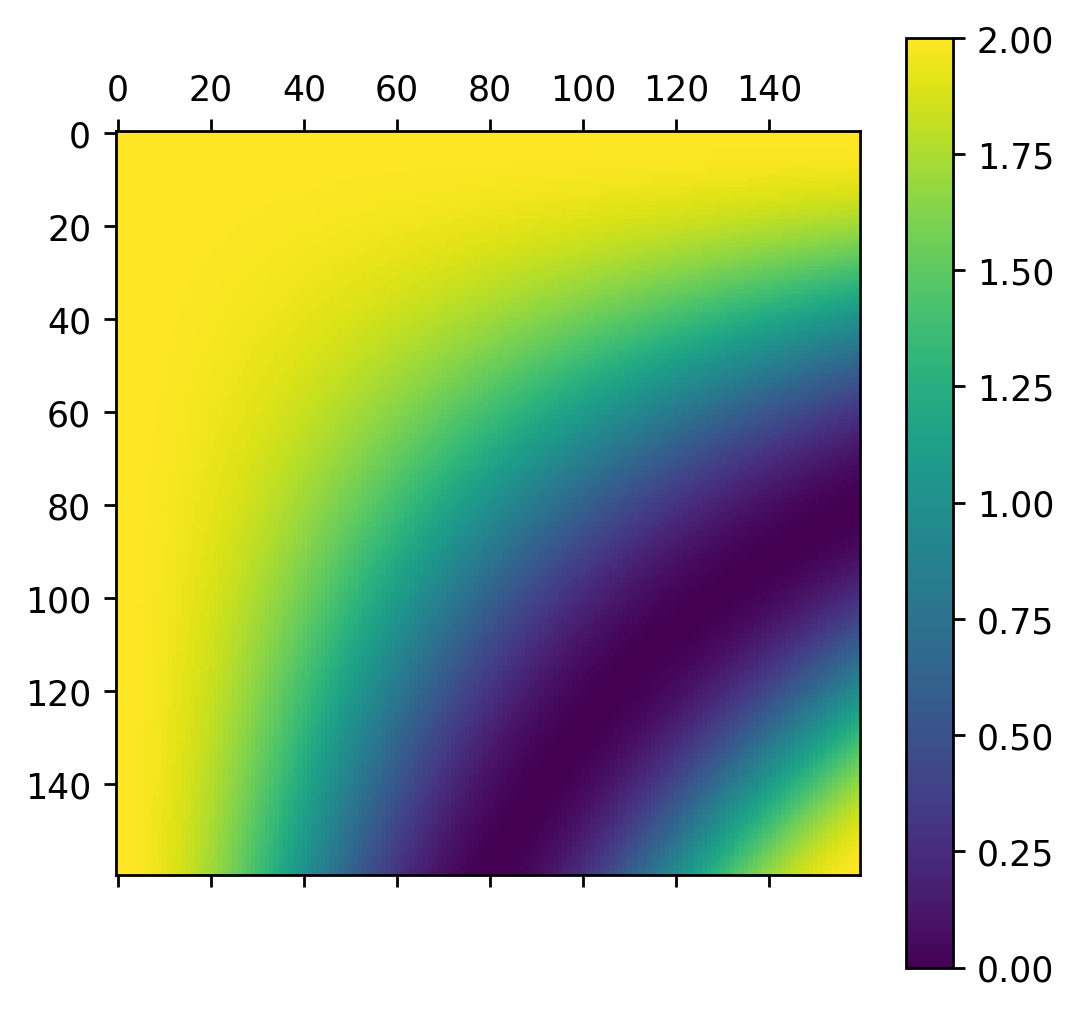
\includegraphics[scale = 0.5]{./figs/160/results_final.png}}
\end{minipage}
\caption{Решение для сетки 160 на 160: слева на 50000 итерации; справа финальное (153615 итерация)}
\end{figure}

\begin{center}
\begin{tabular}{lllllll}
Cores & Threads & Mesh & Time (sec) & Iterations & Error (L2) & Error (C) \\
\hline
4 & 1 & 20 x 20 & 0.017169 & 518 & 0.040182 & 0.005018 \\
4 & 1 & 40 x 40 & 0.188739 & 5007 & 0.019857 & 0.001262 \\
4 & 1 & 80 x 80 & 0.816082 & 33397 & 0.009860 & 0.000316 \\
4 & 1 & 160 x 160 & 7.892072 & 153611 & 0.004905 & 0.000079 \\
\hline
\end{tabular}
\end{center}
Параллельная программа была протестирована на таких же сетках и было проведено сравнение
с последовательной версией. В таблице представлены результаты для параллельной версии.
Видно что ошибки получаются такие же, как для последовательной версии.

\newpage

\subsection{Тестирование на Blue Gene}

Приведем результаты тестирования на суперкомпьютере Blue Gene (\ref{http://hpc.cmc.msu.ru/bgp}). 

В первой таблице показаны результаты тестирования MPI версии программы в режиме VN (режим виртуальных вычислительных узлов).
Программа компилировалась компилятором IBM XL: mpixlcxx -O3 -qarch=450 -qtune=450.
\begin{center}
\begin{tabular}{llllllll}
Cores & Threads & Mesh & Time (sec) & Iterations & Error (L2) & Error (C) & SpeedUp \\
\hline
128 & 1 & 512 x 512 & 736.060111 & 1676500 & 0.001499 & 0.000008 & 1.00 \\	
256 & 1 & 512 x 512 & 464.799801 & 1676433 & 0.001499 & 0.000008 & 1.58 \\
512 & 1 & 512 x 512 & 340.541092 & 1675964 & 0.001499 & 0.000008 & 2.16 \\
\hline
128 & 1 & 1024 x 1024 & 1419.707980 & 1000001 & 192.841024 & 0.375063 & 1.00 \\
256 & 1 & 1024 x 1024 & 770.141615 & 1000001 & 192.841055 & 0.375063  & 1.84 \\
512 & 1 & 1024 x 1024 & 437.776311 & 1000001 & 192.841038 & 0.375063  & 3.24 \\
\hline
\end{tabular}
\end{center}

Во второй таблице показаны результаты тестирования гибридной MPI/OpenMP версии программы в режима SMP (режим симметричного мультипроцессора).
Программа компилировалась компилятором IBM XL: mpixlcx\_r -O3 -qsmp=omp -qarch=450 -qtune=450.
\begin{center}
\begin{tabular}{llllllll}
Cores & Threads & Mesh & Time (sec) & Iterations & Error (L2) & Error (C) & SpeedUp \\
\hline
128 & 4 & 512 x 512 & 685.643375 & 1675906 & 0.001499 & 0.000008 & 1.00 \\
256 & 4 & 512 x 512 & 613.482150 & 1676433 & 0.001499 & 0.000008 & 1.11 \\
512 & 4 & 512 x 512 & 593.274514 & 1675964 & 0.001499 & 0.000008 & 1.15 \\
\hline
128 & 4 & 1024 x 1024 & 669.6818 & 1000001 & 192.841024 & 0.375063 & 1.00 \\
256 & 4 & 1024 x 1024 & 498.4438 & 1000001 & 192.841024 & 0.375063 & 1.34 \\
512 & 4 & 1024 x 1024 & 410.2103 & 1000001 & 192.841024 & 0.375063 & 1.63 \\
\hline
\end{tabular}
\end{center}
Для задачи 1024 на 1024 пришлось поставить ограничение на 10000000 итераций,
иначе задача не успевала посчитаться за лимит по времени (15 минут), за 10000000 итераций
норма невязки успела упасть до 0.82. Для задачи 512 на 512 невязка упала до $\epsilon = 10^{-6}$.
Ускорение считалось относительно времени на 128 ядрах. 

Видно, что для версии MPI - ускорение получается близкое к линейному для задачи 1024 на 1024 узлов. 
Для гибридной версии ускорение получается похуже - возможно это связано с особенностями реализации OpenMP для C++. 

\newpage

\subsection{Тестирование на Polus}

Приведем результаты тестирования на кластере Polus (\ref{http://hpc.cmc.msu.ru/polus}). 

Из-за лимита тестирования по времени на кластере Polus использовалось ограничение по итерациям: 1000000 для задачи 512 на 512 и 100000 для задачи 1024 на 1024.

Приведем результаты тестирования MPI версии программы. Компилирование проводилось 
с использованием компилятора IBM (mpixlC) и флагами: -O3 -qstrict -qarch=pwr8 -qtune=pwr8.
Тестирование проводилось вплоть до максимального лимита по количеству возможных ядер на polus - 64 ядра. Ускорение считалось относительно времени на 4 ядрах.
\begin{center}
\begin{tabular}{llllllll}
Cores & Threads & Mesh & Time (sec) & Iterations & Error (L2) & Error (C) & SpeedUp \\
%\hline
%scaling results
%4  & 1 & 512 x 512 & 1680.4013 & 1000001 & 0.070561 & 0.000275 & 1.00 \\
%16 & 1 & 512 x 512 & 504.0052  & 1000001 & 0.070561 & 0.000275 & 3.33 \\
%32 & 1 & 512 x 512 & 370.455   & 1000001 & 0.070561 & 0.000275 & 4.54 \\
%64 & 1 & 512 x 512 & 231.7093  & 1000001 & 0.070561 & 0.000275 & 7.25 \\
\hline
4 & 1 & 512 x 512 & 1417.981806 & 1000001 & 0.070567 & 0.000275 & 1.00 \\
16 & 1 & 512 x 512 & 393.908352 & 1000001 & 0.070561 & 0.000275 & 3.60 \\
32 & 1 & 512 x 512 & 232.955863 & 1000001 & 0.070569 & 0.000275 & 6.09 \\
64 & 1 & 512 x 512 & 209.950782 & 1000001 & 0.070571 & 0.000275 & 6.75 \\
\hline
4  & 1 & 1024 x 1024 & 568.089891 & 100001 & 1173.411148 & 1.971368 & 1.00 \\
16 & 1 & 1024 x 1024 & 153.858860 & 100001 & 1173.411148 & 1.971368 & 3.69 \\
32 & 1 & 1024 x 1024 & 79.389629  & 100001 & 1173.411148 & 1.971368 & 7.15 \\
64 & 1 & 1024 x 1024 & 63.293906  & 100001 & 1173.411148 & 1.971368 & 8.97 \\
\hline
\end{tabular}
\end{center}

\newpage

\subsection{Профайлинг MPI версии}

Для задачи 1024 на 1024 точек на суперкомьютере Blue Gene был проведен профайлинг MPI версии программы для 512 ядер, 
результаты представлены на рисунке. Также приведено значения ускорения для разных частей параллельной версии по сравнению с последовательной. 

\begin{figure}[htb!]
\begin{minipage}[h]{0.49\linewidth}
\center{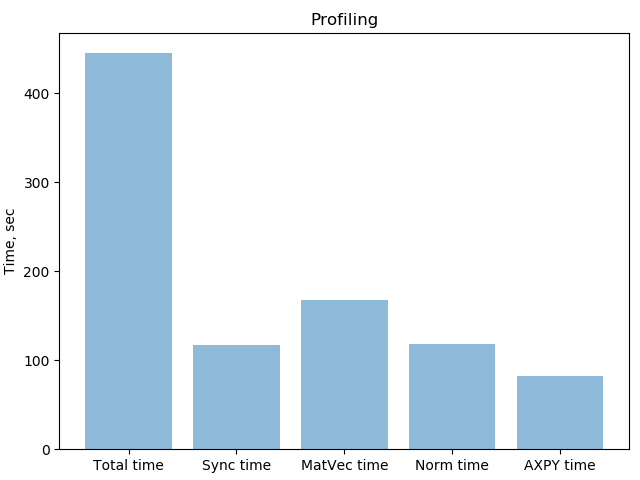
\includegraphics[scale = 0.5]{./figs/profile_MPI_512cores_1024.png}}
\end{minipage}
\hfill
\begin{minipage}[h]{0.49\linewidth}
\center{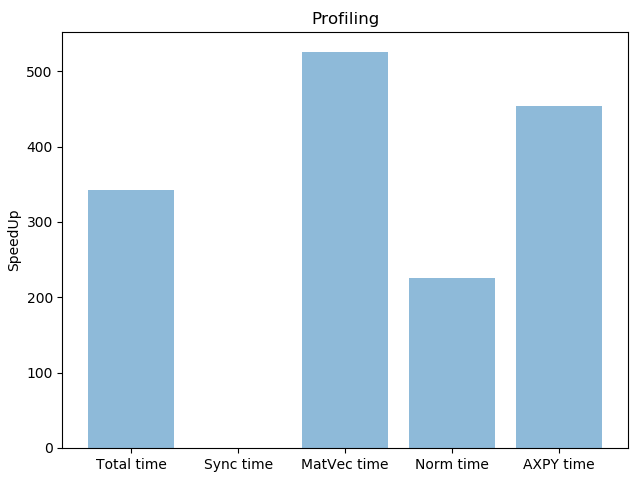
\includegraphics[scale = 0.5]{./figs/profile_speedup_1024.png}}
\end{minipage}
\caption{Слева - время разных частей в программе для параллельной версии на 512 ядрах; справа - ускорение по сравнению последовательной версией. 
Total - общее время; sync - время синхронизаций между процессорами; matvec - время расчета функции "матрица на вектор"; norm - время расчета нормы; 
AXPY - время расчета всех функций вида x = a*x + y}
\end{figure}

Видно, что для операций MatVec и AXPY получается линейное ускорение,
расчет нормы ускоряется хуже в связи с необходимой редукцией для ее расчета. 
\newpage


\section{Заключение}
В рамках данной работы была реализована программа, решающая уравнение Пуассона в прямоугольнике с граничными условиями типа Дирихле и Неймана на границах. 
Была реализована последовательная версия, параллельная MPI версия и гибридная MPI/OpenMP версия. 
Все версии программ были протестированы и показано, что при увеличении сетки в 2 раза ошибка в норме $C$ падает в 4 раза и в норме $L_2$ в 2 раза, как и должно быть согласно теории. 
Параллельные версии были протестированы на суперкомпьютере Blue Gene и кластере Polus. 
На обоих платформах было получено хорошее ускорение, близкое к линейному.

\end{document}
